\section{Irradiation at the Rhode Island Neutron Irradiation Facility}
\label{sec:irradiation}

\subsection{Rhode Island Nuclear Reactor}
\label{subsec:RINSC}
The Rhode Island Nuclear Science Center (RINSC) is a \SI{2}{\mega\watt}, light-water cooled, pool-type reactor in Narragansett, Rhode Island, USA.
Its core consists of fuel assemblies reflected with a combination of graphite and beryllium.
The fuel is plate type U$_3$Si$_2$ cladded with aluminum enriched to less than 20$~\%$ Uranium-235.
At RINSC, there are six different methods to irradiate materials, but only one of these, the 8'' beamport, will be discussed in this paper.
Namely, it is the only sample delivery system large enough to accept full-sized HGCAL silicon sensor wafers and therefore has been revived for this project after its last usage 30 years ago.\newline
A sketch and a photo of the inside of this beamport are shown in \ref{fig:Beamport_Schematic}a and b.
\begin{figure}[!hbt]
  \begin{center}
    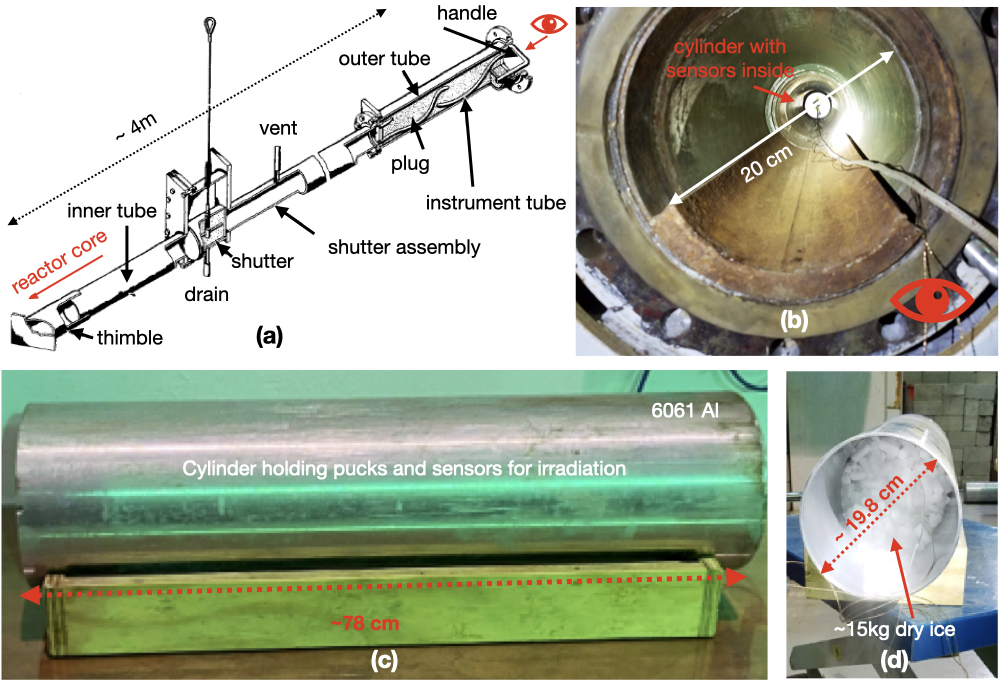
\includegraphics[width=0.99\textwidth]{figures/figures_edited_001.jpeg}
    \caption{(a) Schematic of one of the beamport sample delivery systems at the RINSC Facility.
    (b) The view down into the beamport used for these irradiation studies.
    (c) The sample delivery cylinder that contains the sensor-holding hockey pucks and (d) dry ice for cooling of the silicon sensors during and after irradiation.
    }
    \label{fig:Beamport_Schematic}
  \end{center}
\end{figure}
It measures about \SI{4}{\metre} from the opening to the termination near to the reactor core, and it can accommodate samples with diameters of up to \SI{19.4}{\centi\metre} and a depth of about \SI{90}{\centi\metre}.
A shutter assembly sits \SI{3}{\metre} from the opening of the beamport, which must be raised to allow for the insertion of the experimental setup and closed prior to the start of the reactor.
A \SI{85}{\centi\metre}-long lead plug serves as a radiation shield that has to be inserted into the opening of the beamport prior to the start of irradiation.

\subsection{Irradiation of HGCAL silicon sensor prototypes}
\label{subsec:irradiation}
Given the constraints of the beamport system at RINSC, a dedicated sample delivery method was developed for irradiation HGCAL silicon wafers.
This new sample delivery allows for:
\begin{itemize}
  \item Positioning sensors as close to the reactor core as possible,
  \item protecting them from physical damage during the loading, irradiation, and unloading,
  \item keeping the irradiated sensors at cold temperatures during the after the irradiation,
  \item and monitoring the temperature of the samples inside the reactor.
\end{itemize}
Two compatible pieces of hardware were developed for the irradiation of these silicon sensors: a sensor container, referred to as a hockey puck, and a sample delivery cylinder (see~\ref{fig:Beamport_Schematic}c). 
The former is used to protect, orient, and store the sensors during irradiation while the latter is used to protect and locate the hockey puck inside the beamport.\newline
The cylinder is made from 6061 aluminum, has an outer diameter of \SI{19.5}{\centi\metre} fitting into the beamport, and the inner diameter of the cylinder \SI{18.8}{\centi\metre} allowing for smooth insertion and removal of the hockey pucks.
The cylinder has a welded cap on the end that faces the reactor core and a removable cap with threaded holes for 8 to 32 countersunk flat head machine screws that are flush with the outer wall of the cylinder. 
Both the welded cap and removable cap have vent holes to allow for air to flow into and out of the cylinder.
An eye bolt is screwed into the removable cap to facilitate removing the cylinder from the beamport after irradiations.\newline
The hockey pucks have been made from a variety of different materials including oak, acrylic, and PEEK, see~\ref{fig:Pucks_Arrayed}a. 
\begin{figure}[!hbt]
  \begin{center}
    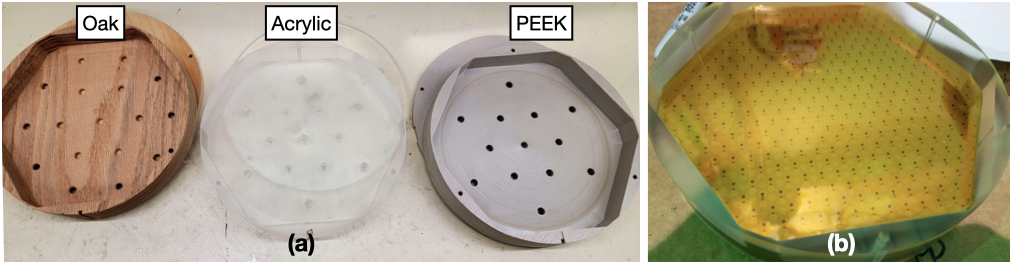
\includegraphics[width=0.99\textwidth]{figures/figures_edited_002.jpeg}
    \caption{(a) Sample containers ('hockey pucks') holding HGCAL silicon sensors for neutron irradiation at RINSC. 
    The deployed materials were wood (oak), acrylic, and PEEK.
    (b) An 8'' high-density HGCAL prototype silicon sensor inside an acrylic puck closed with a Kapton\texttrademark foil.}
    \label{fig:Pucks_Arrayed}
  \end{center}
\end{figure}
The puck base has an outer diameter of \SI{18.6}{\milli\metre} that allows for a smooth fit inside the cylinder. 
Its interior of the puck is milled out in the profile of the silicon sensors with an additional clearance of \SI{1}{\milli\metre}. 
With these constraints the thinnest sections of the wall of the puck are slightly over \SI{1}{\milli\metre} thick which provides a difficult machining challenge.
The puck has a lid, made from the same material as the base, that matches the outer diameter of the base and provides a way to close the puck during handling.
Matching through holes in the base and lid allow for using nylon threaded rods and nuts to fasten the puck together. \newline
Kapton\texttrademark foils were used to separate sensors in a stack such that no sensors are in direct contact with any rough surfaces (cf.~\ref{fig:Pucks_Arrayed}b).
In addition, antistatic foam is used for mechanical protection of the sensors inside the puck.
Sensors were irradiated in batches of four, which required ten layers of Kapton\texttrademark foils and three to four layers of antistatic foam. 
After preparation of the puck it was inserted into the delivery cylinder.
In general, sensors should ideally be kept at low temperatures during the irradiation in order to limit unwanted annealing.
For this purpose, the cylinder was filled with 15-\SI{18}{\kilo\gram} of dry ice.
However, it was found empirically that most of the dry ice is eventually consumed during irradiation.
Therefore, PT1000 resistance temperature detectors (RTD) were inserted into the puck, at the front or back face, to record the temperature throughout the irradiation for assessment of the expected sensor annealing during irradiation.
Before the cylinder was closed, the RTD wires were routed through the vent holes in the removable cap, and were connected to a dedicated temperature readout system outside the beamport.\newline 
Once the cylinder had been fully packed it was loaded onto a sled and inserted into the opening of the beamport.
It was then pushed all the way inside, the shutter was lowered, the lead plug was inserted into the opening of the beamport, and the setup was ready for irradiation.\newline
A representative temperature recording during irradiation is shown in~\ref{fig:Round_10_Temperature_Profile}.
\begin{figure}[!hbt]
  \begin{center}
    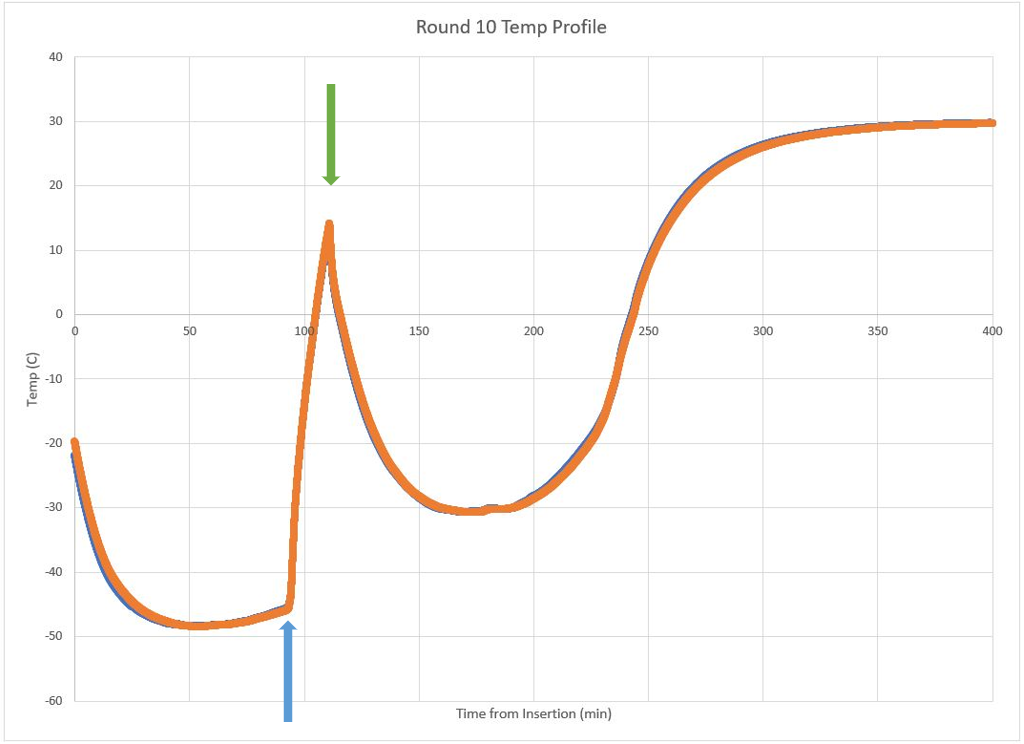
\includegraphics[width=0.60\textwidth]{figures/Round_10_Temperature_Profile}
    \caption{Representative temperature recording during one of the irradiation rounds. 
    The blue arrow indicates the time at when the reactor was turned on, and the green arrow indicates the moment that the reactor was shut off.}
    \label{fig:Round_10_Temperature_Profile}
  \end{center}
\end{figure}
The start up of the reactor takes about 50-\SI{100}{\minute}. 
Once the reactor operated at full capacities, the recorded temperature increased significantly and continued to increase throughout the duration of the irradiation.
As a result, the annealing of the silicon sensors inside the beam port was in fact not negligible.
It varied for the neutron-irradiated sensors between a few minutes to a few hundred minutes equivalent to \SI{60}{\celsius}.
Only after shutdown of the reactor, the temperature decreased again.
After \SI{24}{\hour} in the beamport after irradiation, the cylinder activity decayed sufficiently in order to safely transfer into a storage freezer.

\subsection{Fluence Assessment}

In addition to the sensors, mechanical packing material, and RTDs, each puck contains a number of reference objects for measuring the fluence achieved during an irradiation. 
\iffalse
Three different objects were used to measure the fluences during this campaign: leftover silicon diodes from the D0 experiment, commercially available pin diodes, and ultrapure iron foils. 
After irradiation the iron foils are counted at RINSC and the fluence is calculated based off of the gamma spectrum data.
The irradiated D0 and pin diodes are returned to Brown and measured.
CV and IV measurements are performed to find the depletion voltage and current, then fluence can be estimated using the volume of the diodes and the damage factor of silicon.

The D0 and pin diodes were included inside the puck to measure the fluence as close to the sensors as possible.
To achieve this the diodes were encased in small plastic bags and were taped to the inside faces of the puck. 
The iron foils were attached to the exterior of the cylinder for ease of removal and rapid counting. 

The experience from this campaign has shown that the pin diodes used saturate at low fluences and were not found to be particularly useful in this effort. 
The D0 diodes are most useful at medium-range fluences where the depletion voltage can be measured. 
Many of the D0 diodes irradiated to high fluences did not deplete before 1100V, which is the limit of the power supply used in the measurement setup. 
The iron foils were useful at both the medium and high fluences, but their distance from the silicon made them useful as boundary conditions. 
A table showing the extrapolated fluences from the D0 diodes and iron foils can be found in figure (.~\ref{fig:Round_1_Achieved_Fluences}).

Future irradiations will include iron foils inside the pucks to allow for a more direct comparison with both the irradiated diodes and full sensors. 
Additional test structures will also be included for additional fluence monitoring points.

\subsection{List of Neutron-Irradiated Sensors}

%this could be part of an appendix
\label{subsec:sensors_irradiation}
"Which sensors were irradiated"? \textcolor{red}{Responsible: Thorben}
\begin{itemize}
  \item full table of sensors irradiated in first campaign (see .~\ref{fig:Irradiation_Schedule}). Do we want to include sensors irradiated prior to the main campaign? On the order of 10 or so sensors irradiated prior to this campaign.
\end{itemize}

\begin{figure}[!hbt]
  \begin{center}
    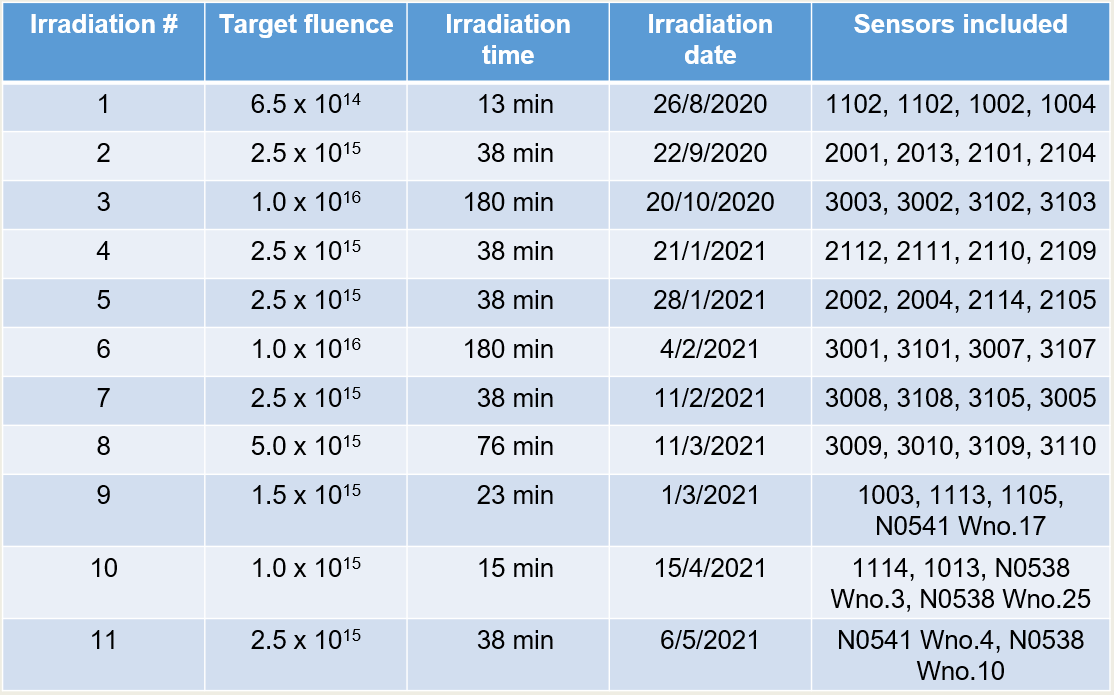
\includegraphics[width=0.90\textwidth]{figures/Completed_Irradiation_Schedule_at_RINSC}
    \caption{Completed irradiation schedule for all sensors irradiated in this campaign.}
    \label{fig:Irradiation_Schedule}
  \end{center}
\end{figure}



\begin{figure}[!hbt]
  \begin{center}
    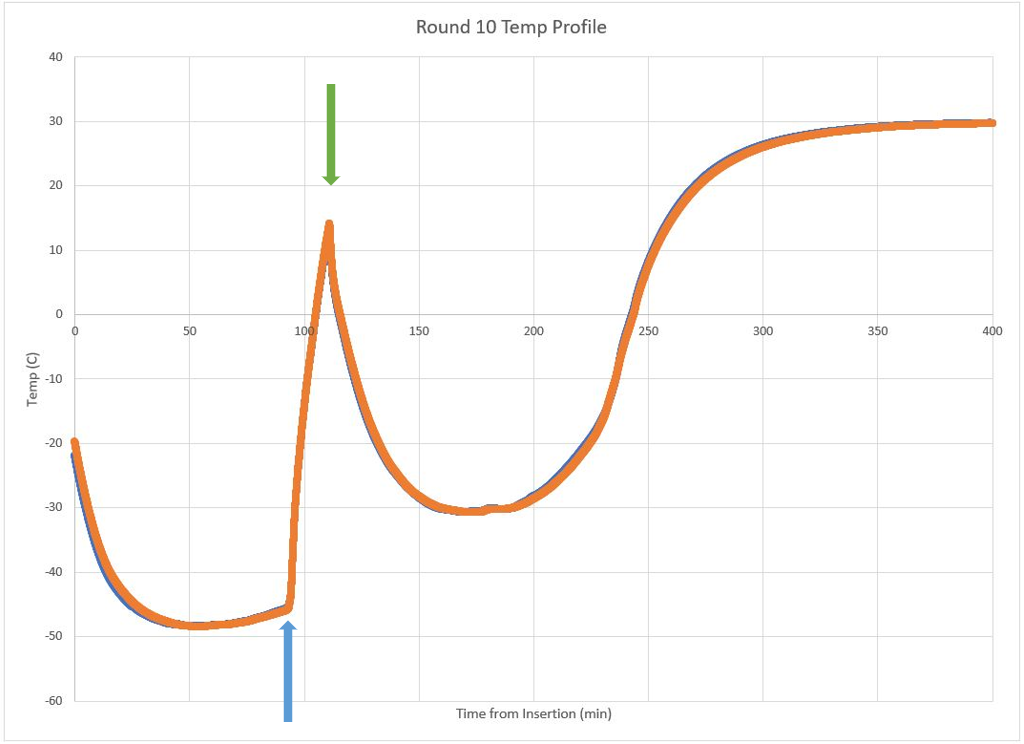
\includegraphics[width=0.80\textwidth]{figures/Round_10_Temperature_Profile}
    \caption{Temperature profile for sensor irradiation round 10. The blue arrow indicates the time at when the reactor was turned on, and the green arrow indicates at what time the reactor was shut off.}
    \label{fig:Round_10_Temperature_Profile}
  \end{center}
\end{figure}

\begin{figure}[!hbt]
  \begin{center}
    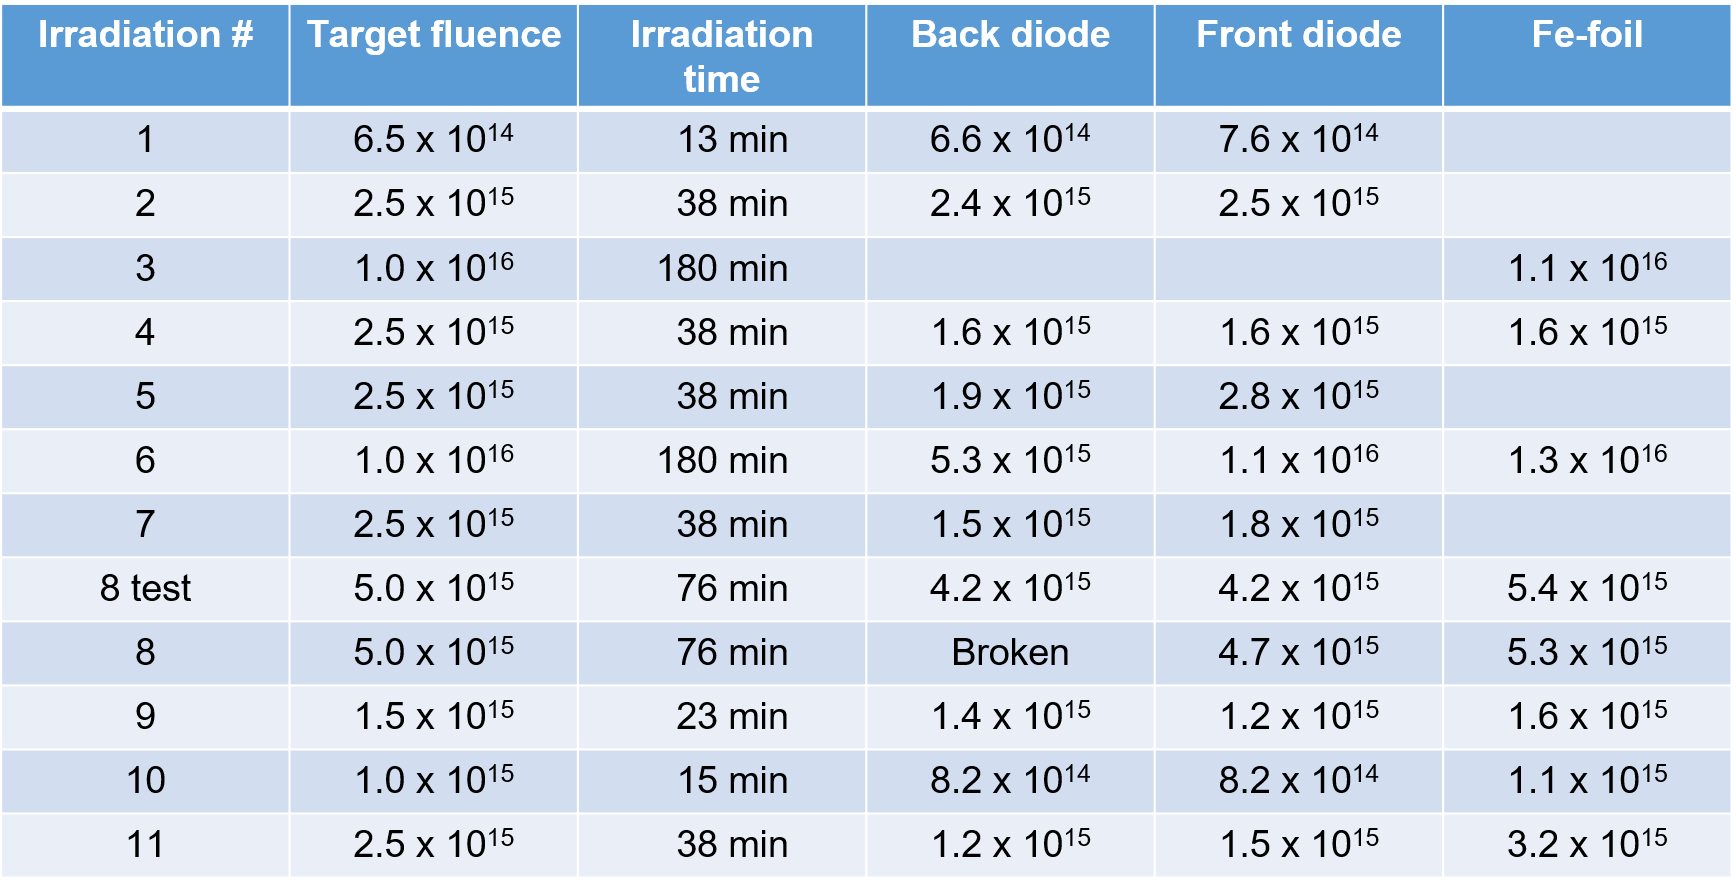
\includegraphics[width=0.80\textwidth]{figures/Round_1_Achieved_Fluences}
    \caption{Table of extrapolated fluences from D0 diodes irradiated alongside full sensors throughout this campaign. Empty cells indicate monitoring diodes or foils that were damaged during handling or not included in specific runs.}
    \label{fig:Round_1_Achieved_Fluences}
  \end{center}
\end{figure}

\begin{itemize}
    \item \ref{fig:RINSC_Facility} - image(s) of reactor core, beamport (see .~\ref{fig:RINSC_Facility})
    %what other details are useful here?
    %Is it better to omit the sample irradiation options that are not being used?
    \item \ref{fig:Pucks_Arrayed} - puck design/layout, real pucks (see .~\ref{fig:Pucks_Arrayed})
    %\item Fig 3 - puck layout, packing (see .~\ref{fig:Puck_Packing}), how much detail about packing materials? (see .~\ref{fig:Cylinder_Details})
    %\item Fig 4 - other hardware, cylinder, temp monitoring setup (see .~\ref{fig:Temperature_Monitoring_Setup})
    %Keithley 2400 for temperature readout (along with 20-channel input board), RTDs instrumented with 20' of radiation-resistant wire (McMaster), laptop with GPIB connection to keithely, and custom LabVIEW code for readout.
    %\item Fig 5 - schemaitc of experimental setup? Is this needed?
    %\item describe sample removal/storage after irradiation - need for full day for activity levels to decay to the point that reactor staff can transfer cylinder from beamport to freezer. Chest freezer has been installed a few steps away from the beamport with enough storage capacity for 3 cylinders.
    %\item Fig 6 describe fluence measurement setup/procedure at Brown? IV of D0 diodes prior to irradiation, then cold (-20C) measurement of irradiated diodes with current scaled up to 20C. Also include pin diodes but they have not been found to be useful at fluences above 1e15. (see .~\ref{fig:Fluence_Measurement_Setup})
    \begin{itemize}
  \item Puck and other hardware for placement of the sensors into the beamport
  \item Temperature (!) as it may cause annealing (affecting the IV+CV results). Usage of dry ice.
  \item Temperature monitoring essential. Show illustrative temperature-vs-time graph during irradiation round. 
\end{itemize}
\end{itemize}

\begin{figure}[!hbt]
  \begin{center}
    \includegraphics[width=0.70\textwidth]{figures/Hockey_Pucks_Arrayed}
    \caption{Sample containers ('hockey pucks') for sensors to be irradiated in the beamport at RINSC. The materials are wood (oak), acrylic, and PEEK.}
    \label{fig:Pucks_Arrayed}
  \end{center}
\end{figure}

\fi
